\documentclass[runningheads]{llncs}
\usepackage{graphicx}
\usepackage{float}
\restylefloat{figure}
\usepackage{xcolor}
\usepackage{listings}
\lstset{
  language=C,                % choose the language of the code
  numbers=left,                   % where to put the line-numbers
  stepnumber=1,                   % the step between two line-numbers.        
  numbersep=5pt,                  % how far the line-numbers are from the code
  backgroundcolor=\color{white},  % choose the background color. You must add \usepackage{color}
  showspaces=false,               % show spaces adding particular underscores
  showstringspaces=false,         % underline spaces within strings
  showtabs=false,                 % show tabs within strings adding particular underscores
  tabsize=2,                      % sets default tabsize to 2 spaces
  captionpos=b,                   % sets the caption-position to bottom
  breaklines=true,                % sets automatic line breaking
  breakatwhitespace=true,         % sets if automatic breaks should only happen at whitespace
  title=\lstname,                 % show the filename of files included with \lstinputlisting;
}
\begin{document}

\title{Monitorizarea traficului(A)}
\author{Damian Alexandru, grupa B5, anul 2}
\institute{Facultatea de informatica Iasi}
\maketitle



\keywords{TCP \and client-server \and threads \and C \and C++}


\section {Introducere}
\subsubsection{Motivatie}
Am ales sa fac acest proiect deoarece am vrut sa aprofundez conceptele de retelistica. Consider ca acest proiect ma va ajuta sa inteleg mai bine cum sunt implementate sistemele de gestiune a traficului, sau aplicatiile folosite pentru navigare.\\

Voi realiza aplicatia in limbajul C si C++ cu o interfata grafica pentru client realizata in Qtcreator.

\section {Tehnologiile utilizate}

In acest proiect voi folosi protocolul TCP/IP deoarece vreau sa fiu sigur ca toti clientii vor primi notificarile pentru evenimente, accidente din zonele in care se afla. Prin utilizarea protocolului TCP/IP, clientul va crea o conexiune stabila cu serverul, astfel transferul de informatii va fi garantat.\\

Pentru a permite accesul mai multor clienti la server in acelasi timp, voi crea un server TCP concurent. Pentru fiecare client conectat, voi crea un nou thread in server.\\

De asemenea, la proiect ma voi folosi si de Qtcreator pentru a realiza interfata clientului.\\


\section{Arhitectura aplicatiei}

Serverul va astepta conexiuni din partea clientilor. Pentru fiecare client, serverul va obtine 2 file-descriptori prin care va comunica cu acel client, si va crea un thread doar pentru acel client. Deci pentru fiecare client, in server va exista cate un thread.\\

Primul fd, va fi pentru comunicarea datelor de logare/inregistrare, si comunicarea optiunilor si incidentelor trimise de client catre server. Al doilea fd, va fi folosit pentru a realiza broadcastul si pentru a citi locatia clientului. Cand un client va trimite o informatie despre un accident, serverul va inregistra aceasta informatie, si va seta o variabila accesibila fiecarui thread astfel incat in fiecare thread va sti ca va trebui sa trimita informatia clientului sau.\\

Drumul unui client va fi stabilit folosind un algoritm dfs. Punctul de start, destinatia si viteza vor fi alese aleator, iar viteza se va actualiza si locatia se vor actualiza o data la 2 secunde. Orice locatie trimisa intre server si client este de forma "STRADA NUMAR". \\

Pentru a simula deplasarera unei masini, in client voi calcula distanta parcursa de client in 2 secunde, la viteza initiala. Din distanta totala a strazii, voi scadea aceasta distanta. Cand un client trimite locatia catre server, server-ul se va uita la strazile care au o legatura cu strada clientului si va trimite evenimentele aferente acelor strazi.

\begin{figure}[H]
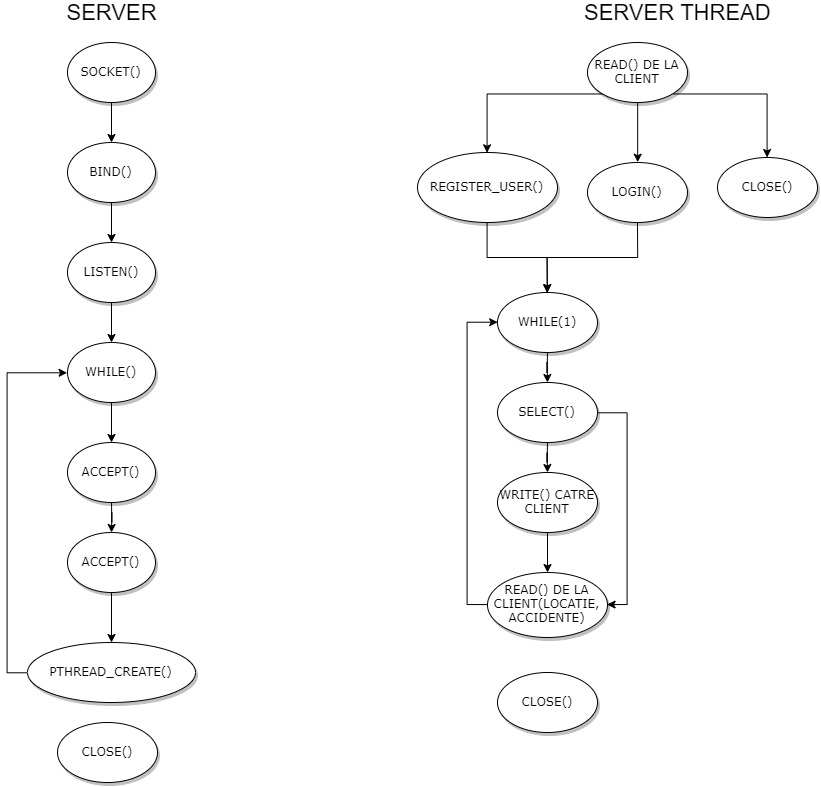
\includegraphics[width=\textwidth]{SERVER_SERVER_THREAD.jpg}
\caption{Diagrama server}
\end{figure}

Clientul va avea un main thread si un listening thread si 2 socketi. Pe primul socket va comunica cu serverul datele de logare, si va introduce introduce date in caz de accident. Al doilea socket, va trimite date la server despre locatia si viteza clientului, si va primi de la server informatii despre limita de viteza, incidente (maracte de alti utilizatori) si evenimentele din acea zona.

Pentru a actualiza interfata clientului, ma voi folosi de sistemul SIGNAL - SLOT din QT. Astfel, cand voi primi o informatie noua in thread-ul de ascultare (listening thread) voi emite un semnal care va fi receptionat in client, unde va fi actualizata interfata.
\begin{figure}[H]
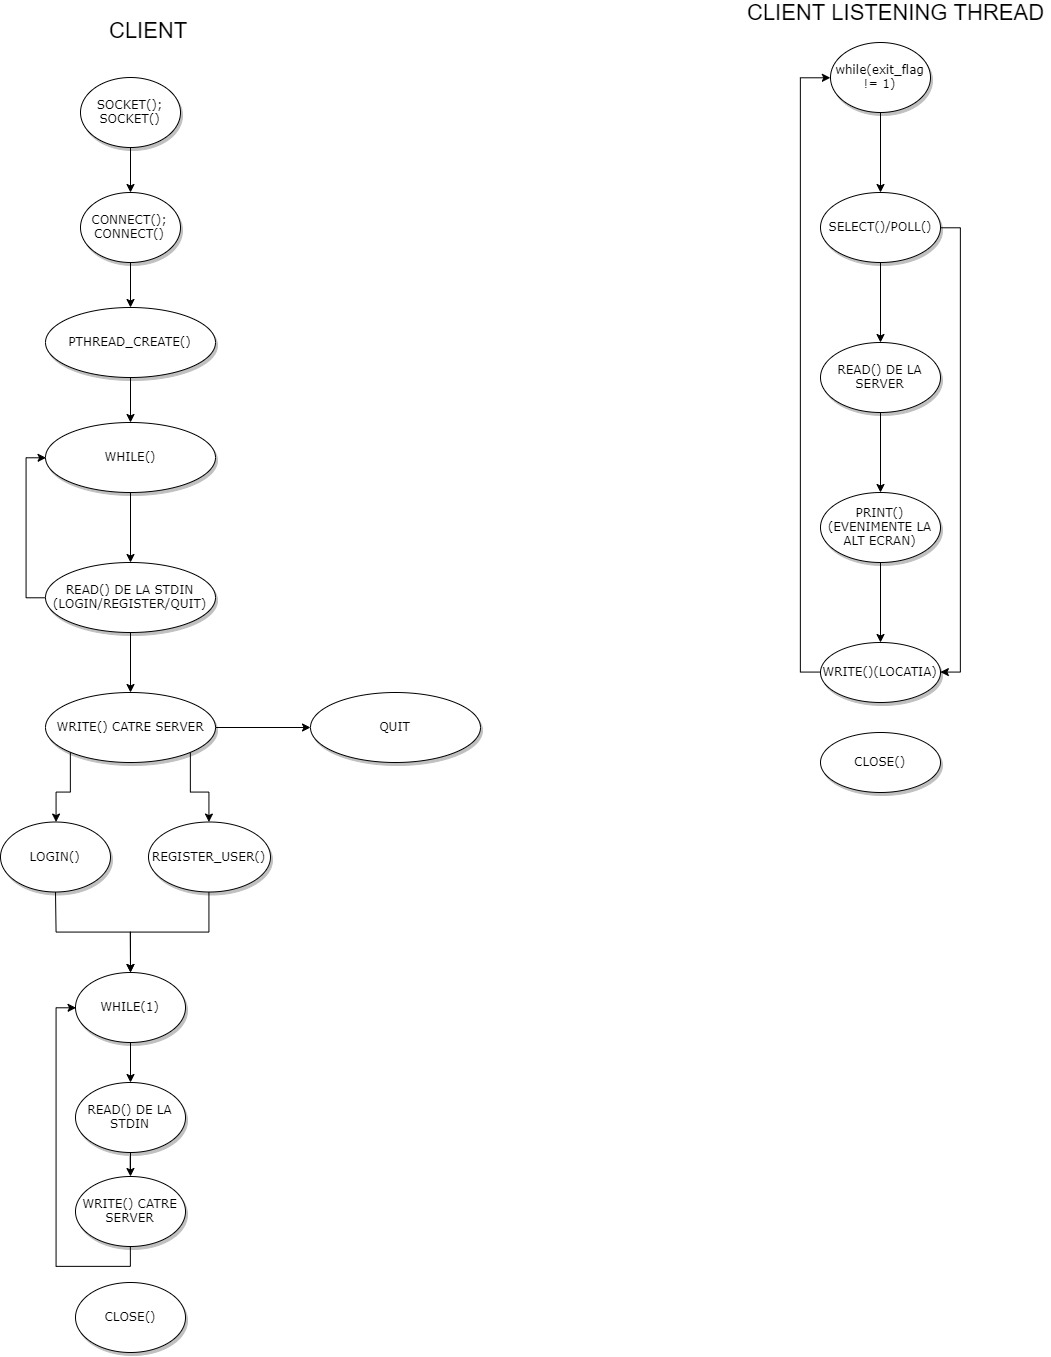
\includegraphics[width=\textwidth]{CLIENT_CLIENT_THREAD.jpg}
\caption{Diagrama client}
\end{figure}
Clientul va avea un loc in care poate introduce "accident" sau diferite comenzi. De asemenea va avea si o lista care va fi actualizata cu evenimentele din jurul sau in timp real.\\

Pentru a simula strazile unui oras, voi folosi un graf. Acesta va fi retinut sub forma unui vector de muchii. Clientii se vor deplasa de la un nod x la un nod y. Aceste noduri vor fi alese aleator la inceput, iar drumul va fi ales folosind un dfs. Zonele cu restrictie de viteza, evenimentele si accidentele vor fi retinute de server intr-un vector de structuri, iar locatia lor va fi retinuta ca "Nume\_strada numar\_de\_pe\_strada".


\begin{figure}[H]
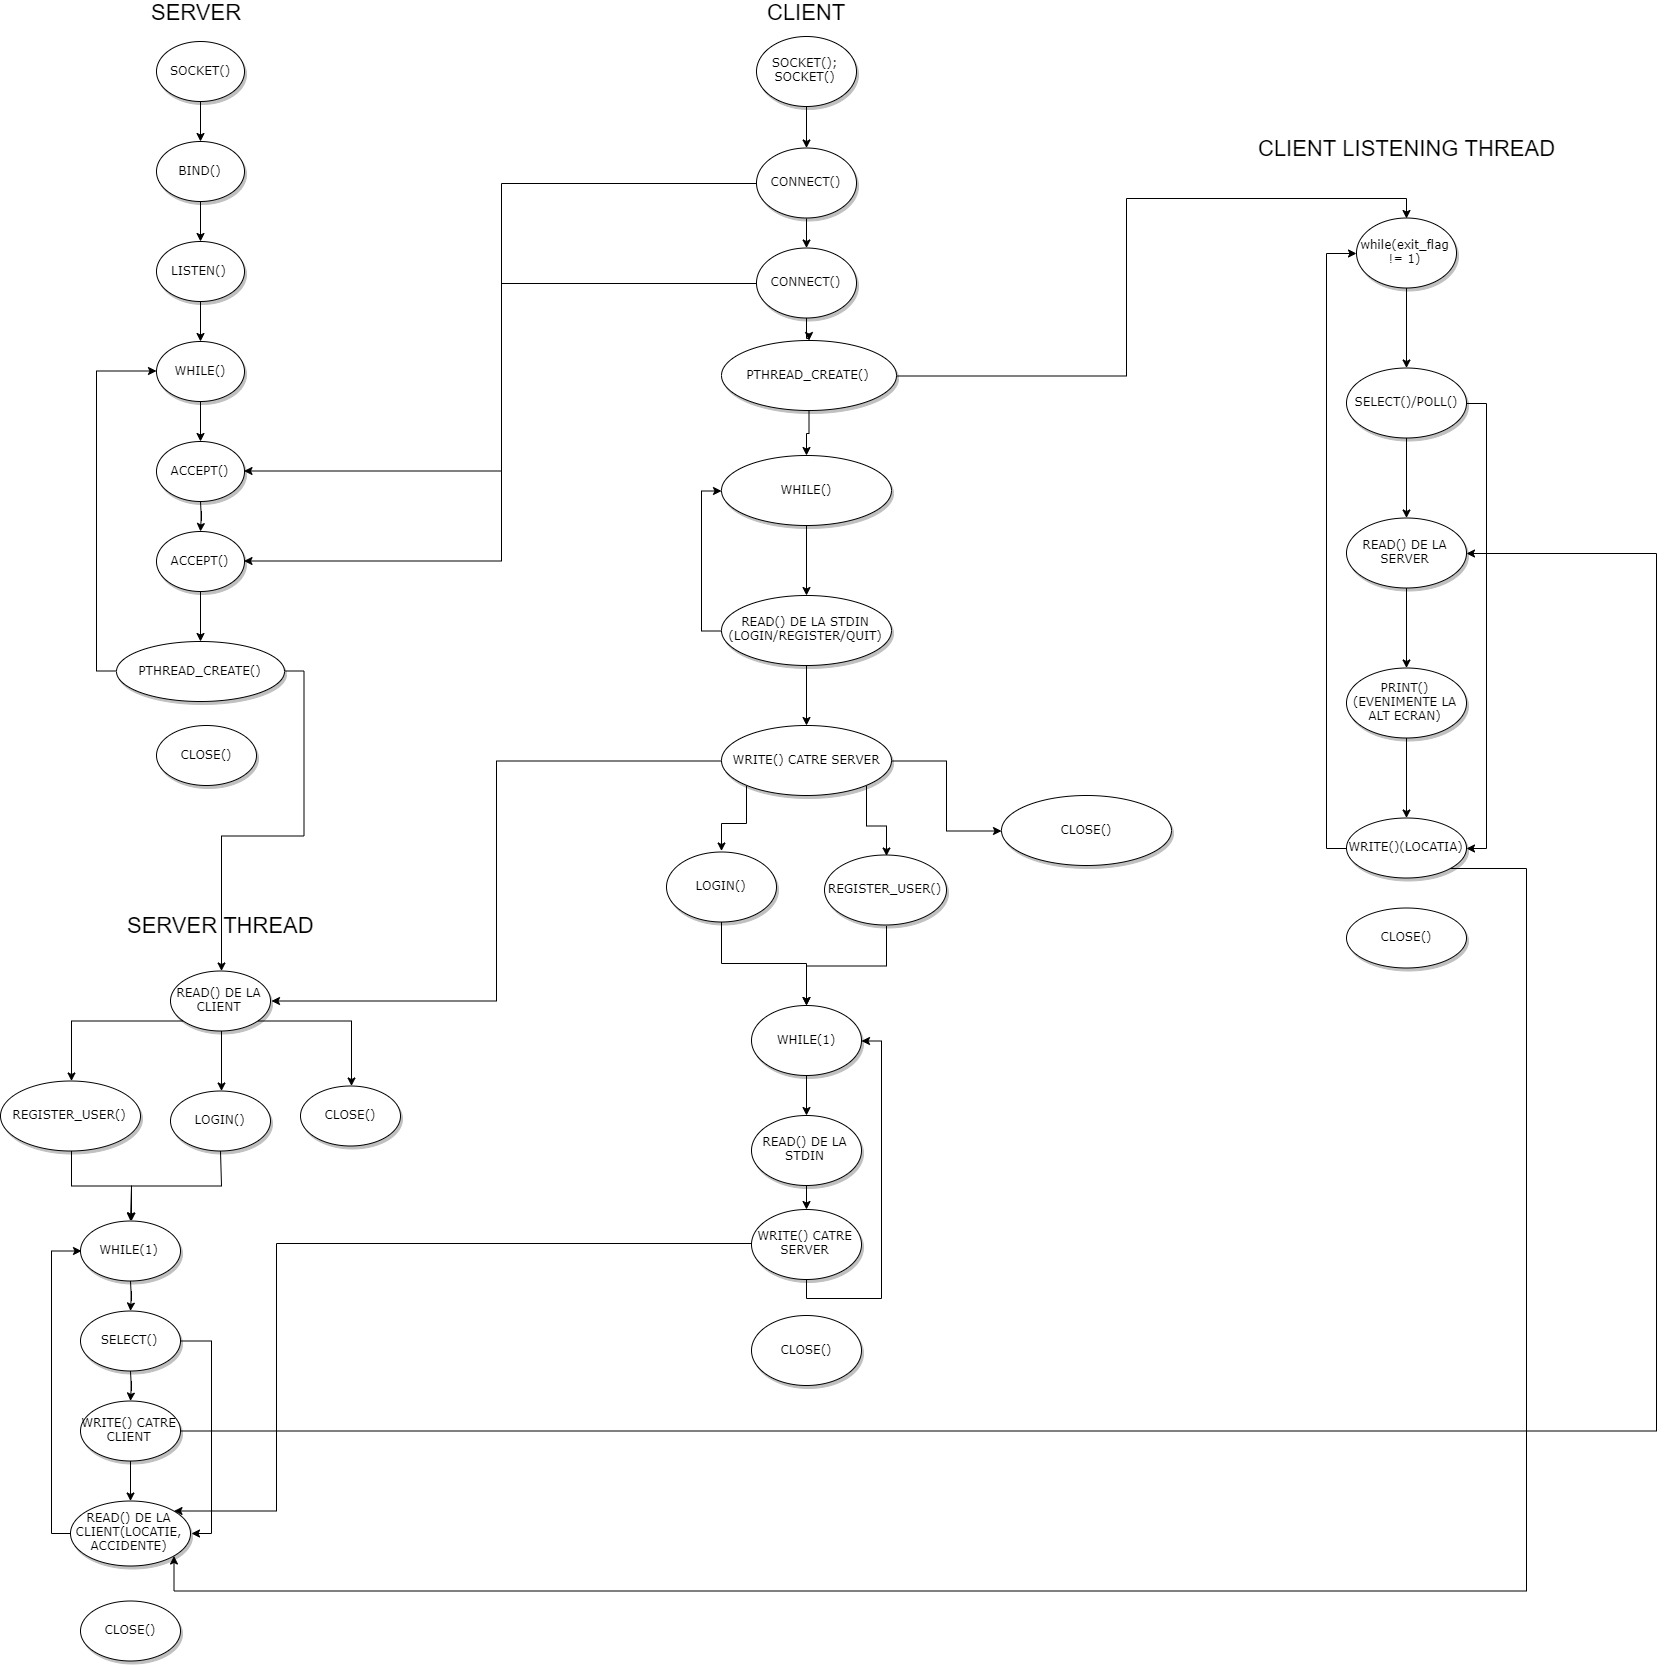
\includegraphics[width=\textwidth]{APPLICATION.jpg}
\caption{Diagrama generala a aplicatiei}
\end{figure}

\begin{figure}[H]
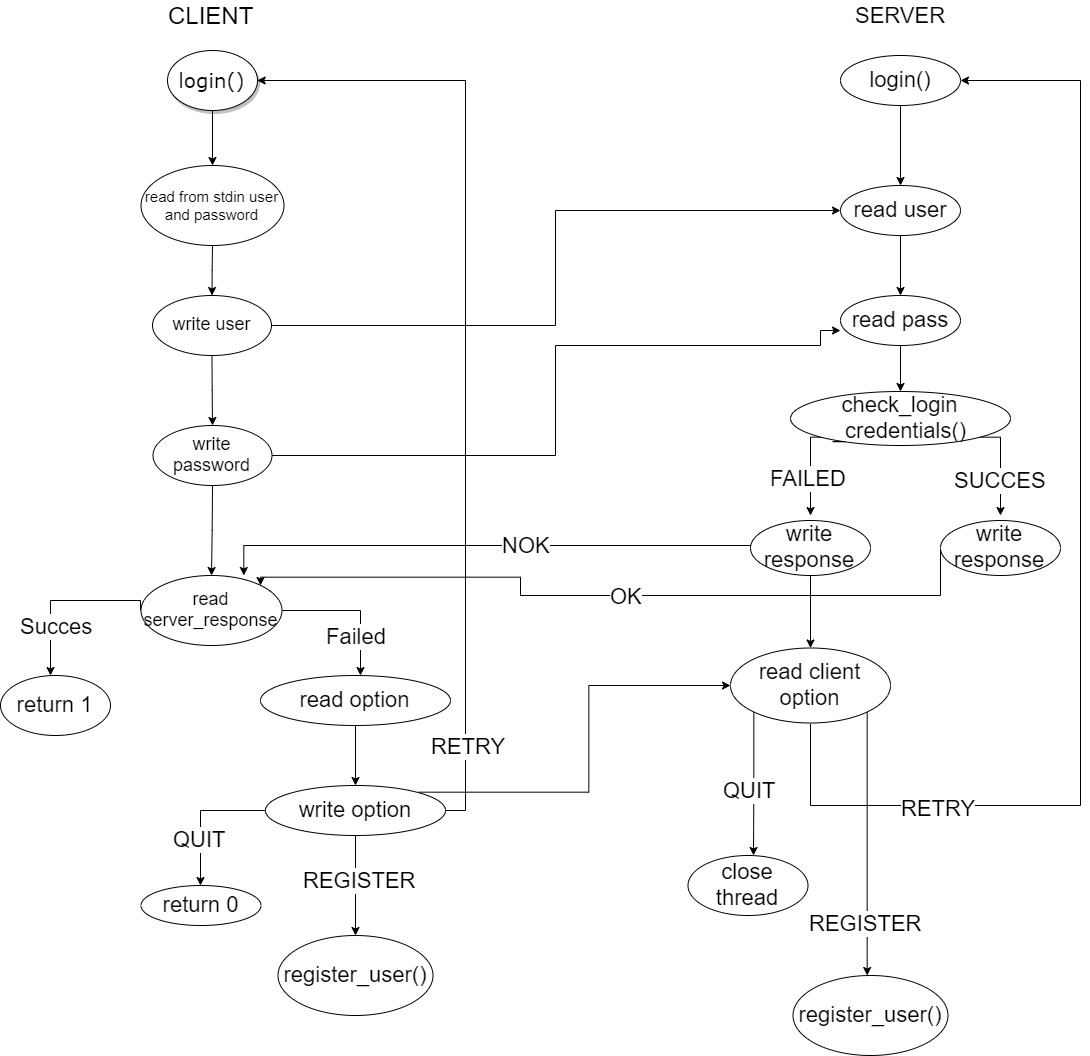
\includegraphics[width=\textwidth]{login.jpg}
\caption{Functia login}
\end{figure}

\begin{figure}[H]
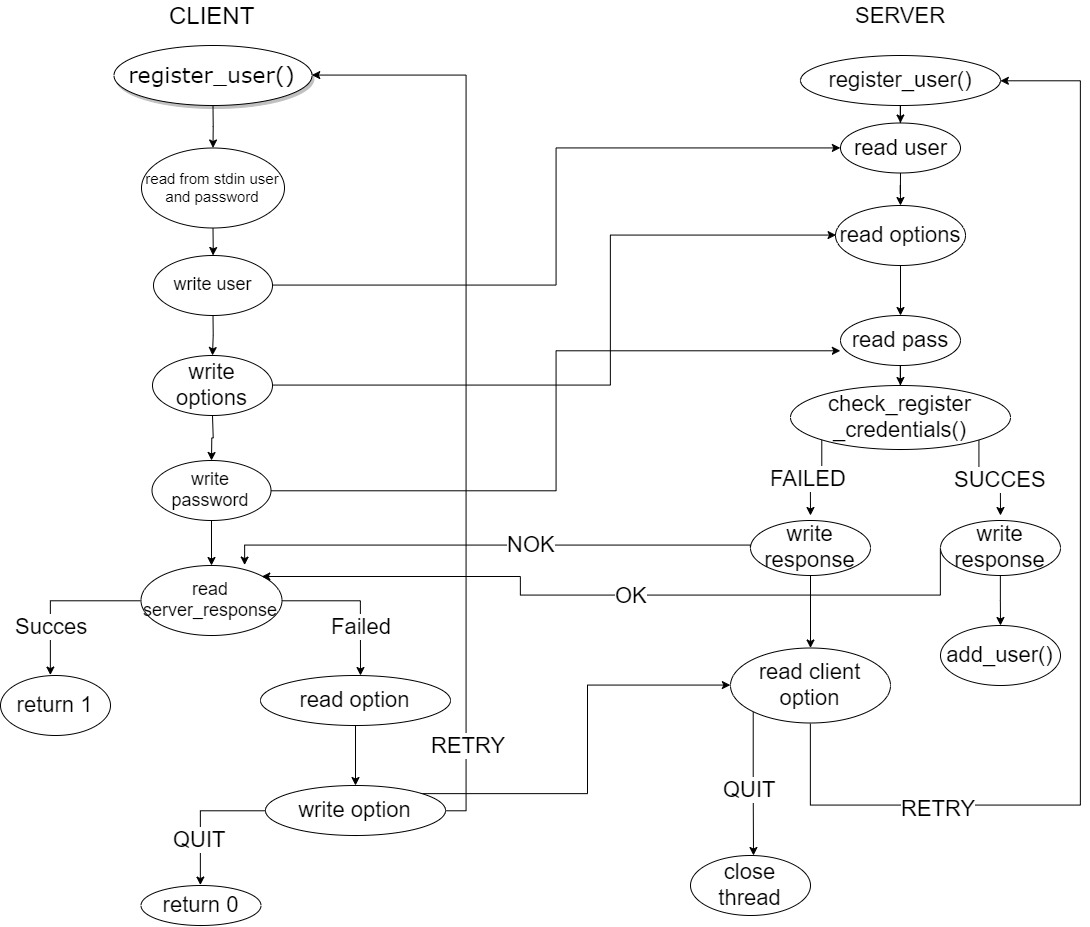
\includegraphics[width=\textwidth]{register.jpg}
\caption{Functia register}
\end{figure}

\section {Detalii de implementare}
Clientul va avea de ales intre register, login si quit. Daca se va inregistra, acesta va trebui sa isi aleaga si evenimentele pe care vrea sa le primeasca(informatii despre vreme, evenimente sportive, preturi pentru combustibili la statiile peco). Dupa ce conectarea s-a realizat cu succes, clientul va putea sa introduca accident sau inchide. Daca introduce accident locatia va fi luata automat si transimsa catre server.\\
\begin{figure}[H]
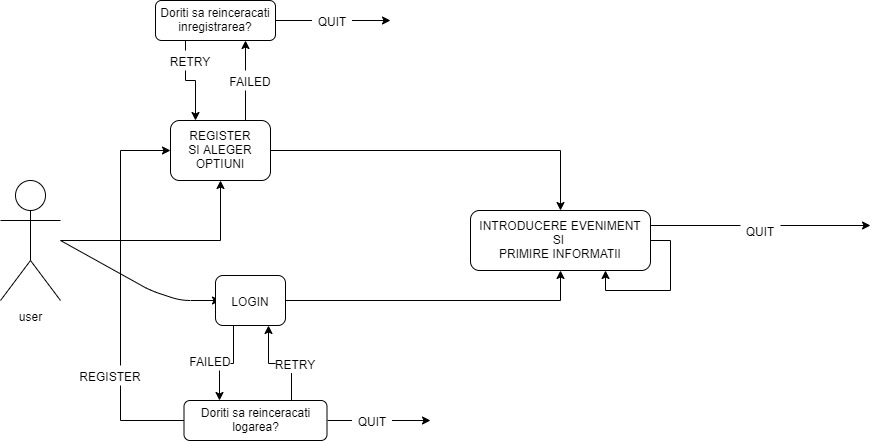
\includegraphics[width=\textwidth]{use-case.jpg}
\caption{Cum va folosi clientul aplicatia}
\end{figure}
Functia de login din server
\begin{lstlisting}
int login(int sd, int id, char options[4]){
    char credentials[100];
    if(read(sd, credentials, 100) < 0){
        perror("Eroare la citire mesaj");
        return -1;
    }
    

    /// check ///
    int check_code;
    if(strlen(credentials) <= 2){
        check_code = 0;
    }
    else check_code = check_login_credentials(credentials, options);
    if(check_code == 0){
        if(write(sd, "NOT OK", 7) < 0){
            perror("Eroare la scriere mesaj");
            return -1;
        }
        printf("[thread \%d]Clientul nu s-a logat cu succes!\n", id);
        return 0;
    }else if(check_code == 1){
        if(write(sd, "OK", 3) < 0){
            perror("Eroare la scriere mesaj");
            return -1;
        }
        printf("[thread \%d]Clientul s-a logat cu succes!\n", id);
        return 1;
    }
    return 0;
}
\end{lstlisting}
Functia de login din client
\begin{lstlisting}
bool Client::conn(){//the listening thread will start after the connection was established
    this->listen_socket = socket(AF_INET, SOCK_STREAM, 0);
    this->info_socket = socket(AF_INET, SOCK_STREAM, 0);
    struct sockaddr_in server;

    server.sin_addr.s_addr = inet_addr("127.0.0.1");
    server.sin_port = htons(2038);
    server.sin_family = AF_INET;

    int conn_code = ::connect(this->info_socket, (struct sockaddr*)&server, sizeof(struct sockaddr));
    int conn_code2 = ::connect(this->listen_socket, (struct sockaddr*)&server, sizeof(struct sockaddr));

    if(conn_code == -1 || conn_code2 == -1){
        ui->listWidget->addItem("Eroare la stabilire conexiune!");
        return false;
    }

    form = new Dialog(this, info_socket);
    int connect = form->exec();
    if(connect == 1){
        ui->listWidget->addItem("Conectare reusita!");
        ui->listWidget->addItem("Bine ati venit!");
        ui->listWidget->addItem("Aici veti primi informatii relevante locatiei curente.");
        lThread->setDescriptor(listen_socket);
        lThread->start();
        return true;
    }
    return false;

}

\end{lstlisting}
Functia register user din server
\begin{lstlisting}
void register_user(int sd, int id){
    /// check ///
    while(1){
        char user[INPUT_SIZE]; 
        char pass[INPUT_SIZE]; 
        read(sd, user, INPUT_SIZE);
        read(sd, pass, INPUT_SIZE);
        int check_code = check_register_credentials(user, pass);
        printf("code = \%d\n", check_code);
        if(check_code == 1){
            write(sd, "NOT OK", 7);
            //vezi ce a trimis clientul
            char option[100];
            read(sd, option, 100);
            if(strcmp(option, "quit") == 0){
                check_code = -1;
                break;
            }else if(strcmp(option, "retry") == 0){
                continue; //bucla while va merge inca o data
            }
        }else if(check_code == 0){//add user
            add_user(user, pass);
            printf("[thread \%d]Clientul \%s s-a inregistrat cu succes!\n", id, user);
            write(sd, "OK", 3);
            break;             
        }
    }
}
\end{lstlisting}
Functia check login credentials din server
\begin{lstlisting}
int check_login_credentials(char*credentials, char options[4]){// -1 daca e eroare, 1 daca am gasit user + pass, 0 altfel
    char user[50], pass[50];
    int k = 0, m = 0;
    while(credentials[k] != '&'){
        user[k] = credentials[k];
        k++;
    }
    user[k] = '\0';

    while(credentials[k] == '&'){
        k++;
    }
    while(credentials[k] != '&' && k < strlen(credentials)){
        pass[m++] = credentials[k++];
    }
    pass[m] = '\0';

    int fd = open("useri.txt", O_RDWR);
    if(fd < 0){
        perror("Eroare la deschidere fisier");
        return -1;
    }
    int found = 0;
    k = 0;
    char word1[110];

    while(!found){//parcurg fisierul
        unsigned char ch;
        int codr = read(fd, &ch, 1);
        if(codr == 0){  //end of file
            break;
        }else if(codr == -1){
            perror("Eroare la citire");
            close(fd);
            return -1;
        }
        if(ch != ' ' && ch != '\n'){//obtinem user-ul de pe o linie
            word1[k++] = ch;
        }
        if(ch == ' '){
            word1[k] = '\0';
            if(strcmp(word1, user) != 0){//daca e un user diferit, sarim linia
                while(ch != '\n'){//parcurgem linia pana la sfarsit
                    read(fd, &ch, 1);
                }
                k = 0;
            }else{ // daca am gasit user-ul verificam parola
                int t = 0;
                char password[50];

                read(fd, &ch, 1);
                password[t++] = ch;
                while(ch != ' '){//obtinem parola
                    read(fd, &ch, 1);
                    password[t++] = ch;
                }
                password[t-1] = '\0';

                if(strcmp(pass, password) == 0){//verificam parola
                    //daca parola este buna, vom citi optiunile
                    
                    for(int o = 0; o < 3; o++){
                        read(fd, &ch, 1);
                        options[o] = ch;
                    }
                    options[3] = '\0';
                    close(fd);
                    return 1;
                }
                while(ch != '\n'){//parcurgem linia pana la sfarsit
                    read(fd, &ch, 1);
                }
                k = 0;
            }
        }
    }
    close(fd);
    return found;
}

\end{lstlisting}
Functia care obtine evenimentele din zona unei locatii
\begin{lstlisting}
char* get_events(char*street_name, int number_on_street, int event_sent[100], char options[4]){
    int found = 0, ref_number;
    //obtinere indicele strazii clientului din vectorul strada[]
    for(int i = 0; i < nr_strazi && found == 0; i++){
        if(strcmp(strada[i].nume, street_name) == 0 
            && number_on_street >= strada[i].nr_locuinte[0]                                    
            && number_on_street <= strada[i].nr_locuinte[1]){
                found = 1;
                ref_number = i;
            }
    }
    char*events = (char*)malloc(200);
    events[0] = '\0';
    strcat(events, "limita:");
    strcat(events, itoa(strada[ref_number].limita));
    strcat(events, "&&");
    int k;
    char**neighbours = get_neighbours(ref_number, &k);
    for(int i = 0; i < total_events; i++){
        for(int j = 0; j < k; j++){//verifica vecinii
            if(strcmp(event[i].street, neighbours[j]) == 0 && event_sent[i] == 0){//caut un eveniment netrimis situat in apropiere

                if(event[i].type[0] == 1 && options[0] == '1'){//vreme
                    strcat(events, "Vreme:");
                    strcat(events, event[i].message);
                    strcat(events, " pe strada ");
                    strcat(events, event[i].street);
                    if(event[i].number != -1){
                        strcat(events, " nr. ");
                        strcat(events, itoa(event[i].number));
                    }
                    strcat(events, "&&");
                    event_sent[i] = 1;
                }else if(event[i].type[1] == 1 && options[1] == '1'){//sport
                    strcat(events, "Sport:");
                    strcat(events, event[i].message);
                    strcat(events, " pe strada ");
                    
                    strcat(events, event[i].street);
                    if(event[i].number != -1){
                        strcat(events, " nr. ");
                        strcat(events, itoa(event[i].number));
                    }
                    strcat(events, "&&");
                    event_sent[i] = 1;
                }else if(event[i].type[2] == 1 &&options[2] == '1'){//pret
                    strcat(events, "Pret statie peco:");
                    strcat(events, event[i].message);
                    strcat(events, " pe strada ");
                    
                    strcat(events, event[i].street);
                    if(event[i].number != -1){
                        strcat(events, " nr. ");
                        strcat(events, itoa(event[i].number));
                    }
                    strcat(events, "&&");
                    event_sent[i] = 1;
                }
            }
        }
    }
    return events;
}
\end{lstlisting}
Un thread din server
\begin{lstlisting}
void* routine(void*arg){
    thData thread = *((thData*)arg);
    int sd = thread.client_fd;
    printf("[thread \%d]Thread inceput.\n", thread.thread_id);
    char options[3];
    int idf = identify(sd, thread.thread_id, options);
    if(idf == -1){
        printf("[thread \%d] Inchidere thread.\n", thread.thread_id);
        close((uintptr_t)arg);
        return NULL;
    }
    char msg[100];
    int broadcast_descriptor = thread.broadcast_fd, quit = 0;
    int nr_accidente_din_thread = 0;
    int client_speed = 0;
    struct pollfd fds[1];
    memset(fds, 0, sizeof(fds));
    fds[0].fd = sd;
    fds[0].events = POLLIN;

    struct pollfd location_fd[1];
    memset(location_fd, 0, sizeof(location_fd));
    location_fd[0].fd = broadcast_descriptor;
    location_fd[0].events = POLLIN;


    int time = 2000;//2 seconds;
    int event_sent[100];
    for(int i = 0 ; i < 100; i++){
        event_sent[i] = 0;
    }
    while(quit == 0){
        printf("[thread \%d] Stau si ascult evenimente de la client\n", thread.thread_id);
        
        int poll_code = poll(fds, 1, time); //al doilea parametru e folosit pentru a spune cate elemente are multimea de descriptori
        if(poll_code < 0){
            perror("Eroare la poll");
            break;
        }
        if(poll_code == 0){//timeout
            printf("[thread \%d]accident poll timedout\n", thread.thread_id);
        }
        else {//s-a intamplat ceva pe socket
            memset(msg, 0, 100);
            int codr = read(fds[0].fd, msg, 100);
            if(codr < 0){
                if(errno != EWOULDBLOCK){
                    perror("Eroare la citire din socket");
                    break;
                }
            }else if(codr == 0){
                printf("[thread \%d] Conexiune inchisa de catre client\n", thread.thread_id);
                break;
            }


            printf("[thread \%d] am primit de la client mesajul >\%s<\n", thread.thread_id, msg);
            //mesajele primite de la client catre server tratate aici sunt de tipul fi de tipul
            // "accident&&nume_strada nr_de_pe_strada
            if(strcmp(msg, "quit") == 0){
                quit = 1;
                break;
            }else{
                char*x = strtok(msg, "&&");
                x = strtok(NULL, "&&");
                accidente[nr_total_accidente].locatie = (char*)malloc(512);
                strcpy(accidente[nr_total_accidente].locatie, x);
                nr_total_accidente++;
            }

            
        }
        char*total_accidente = (char*)malloc(2048);
        total_accidente[0] = '\0';
        while(nr_accidente_din_thread < nr_total_accidente){//la accidente trimit la toti clientii indiferent de locatia lor
            strcat(total_accidente, "Accident:");
            strcat(total_accidente,  accidente[nr_accidente_din_thread].locatie);
            strcat(total_accidente, "&&");
            nr_accidente_din_thread++;
        }
        printf("[thread \%d] nr accidente din thread = \%d, nr total = \%d\n", thread.thread_id, nr_accidente_din_thread, nr_total_accidente);
        printf("[thread \%d] scriu catre client >\%s<\n", thread.thread_id, total_accidente);
        if(write(broadcast_descriptor, total_accidente, strlen(total_accidente)) < 0){
            perror("Eroare la write");
            quit = 1;
            break;
        }

        //astepta locatia trimisa de client
        poll_code = poll(location_fd, 1, 1000);
        if(poll_code == 1){//clientul a trimis locatia sau un cod de succes, daca a ajuns la destinatie
            memset(msg, 0, 100);
            int codr = read(location_fd[0].fd, msg, 100);
            
            if(codr <= 0){
                if(errno != EWOULDBLOCK){
                    perror("Eroare la citire din socket");
                    break;
                }
            }
            if(strcmp(msg, "Succes") == 0){//clientul a ajuns la destinatie
                quit = 1;
            }else{
                char* aux = (char*)malloc(100);
                memset(aux, 0, 100);
                strcpy(aux, msg);
                char * x = (char*)malloc(100);
                strcpy(x, strtok(aux, "&&"));
                client_speed = atoi(x);
                strtok(NULL, "&&");
                char*street = strtok(NULL, "&&");
                char*number = strtok(NULL, "&&");
                int i = 0;
                while(number[i] <= '9' && number[i] >= '0' && i <= strlen(number))i++;
                number[i] = '\0';

                int street_number = atoi(number);
                printf("[thread \%d] viteza client = \%d, locatie client = \%s \%d\n", thread.thread_id, client_speed, street, street_number);
                char* events = get_events(street, street_number, event_sent, options);//TODO adauga parametru si options(alea alese de utilizator la inregistrare)
                printf("[thread \%d] scriu catre client \%s\n", thread.thread_id, events);
                if(write(broadcast_descriptor, events, strlen(events) + 1) < 0){
                    perror("Eroare la write");
                    quit = 1;
                    break;
                }
            }
        }
    }
    
    

    printf("[thread \%d] Inchidere thread\n", thread.thread_id);;
    total_threads--;
    close(broadcast_descriptor);
    close(sd);
    close((uintptr_t)arg);
    return NULL;
}

\end{lstlisting}

\section {Concluzii}

Acest proiect poate fi imbunatatit prin implementarea unei interfete grafice care sa afiseze o harta actualizata in timp real. De asemenea, daca s-ar putea modifica optiunile alese de clienti si dupa ce s-au inregistrat, utilizatorii ar avea parte de o experienta mai buna a aplicatiei.\\

In loc sa folosesc 2 socketi, as putea sa folosesc unul singur daca as adauga noi reguli in comunicare client-server astfel incat sa trimit la un interval de n secunde toate mesajele(accident, eveniment, etc). Acest lucru se poate realiza, daca as pune intr-o coada mesajele care se aduna in acel interval de timp. \\

Pentru a imbunatati viteza serverului, as putea sa apelez functia accept() in threaduri, adica sa fac un threadpoll, sau as putea sa implementez un server TCP prethreaded.
\\
\\
\section {Bibliografie}
\begin{thebibliography}{8}
\bibitem{ref_url1}
\url{https://www.ibm.com/support/knowledgecenter/en/ssw\_ibm\_i\_71/rzab6/poll.htm}
\bibitem{ref_url1}
\url{https://profs.info.uaic.ro/~computernetworks/files/NetEx/S12/ServerConcThread/servTcpConcTh2.c}
\bibitem{ref_url1}
\url{https://profs.info.uaic.ro/~computernetworks/files/NetEx/S12/ServerConcThread/cliTcpNr.c}
\bibitem{ref_url1}
\url{https://profs.info.uaic.ro/~computernetworks/files/7rc\_ProgramareaInReteaIII\_Ro.pdf}
\bibitem{ref_url1}
\url{https://www.qt.io/}
\bibitem{ref_url1}
\url{https://www.youtube.com/playlist?list=PL2D1942A4688E9D63}
\bibitem{ref_url1}
\url{https://profs.info.uaic.ro/~computernetworks/cursullaboratorul.php}
\bibitem{ref_url1}
\url{https://doc.qt.io/}

\end{thebibliography}

\end{document}


